\legend

    We are on a Numeric planet where everything depends on numbers, and we are now on a numbers holiday.

    So the government created a special system to make citizens feel happy and grateful.
    The system was like the following :

    You have $9$ special gifts numbered from $1$ to $9$ and have $2$ big boxes and a numeric board as the following:

    \begin{center}
        \def \htmlPixelsInCm {45}
        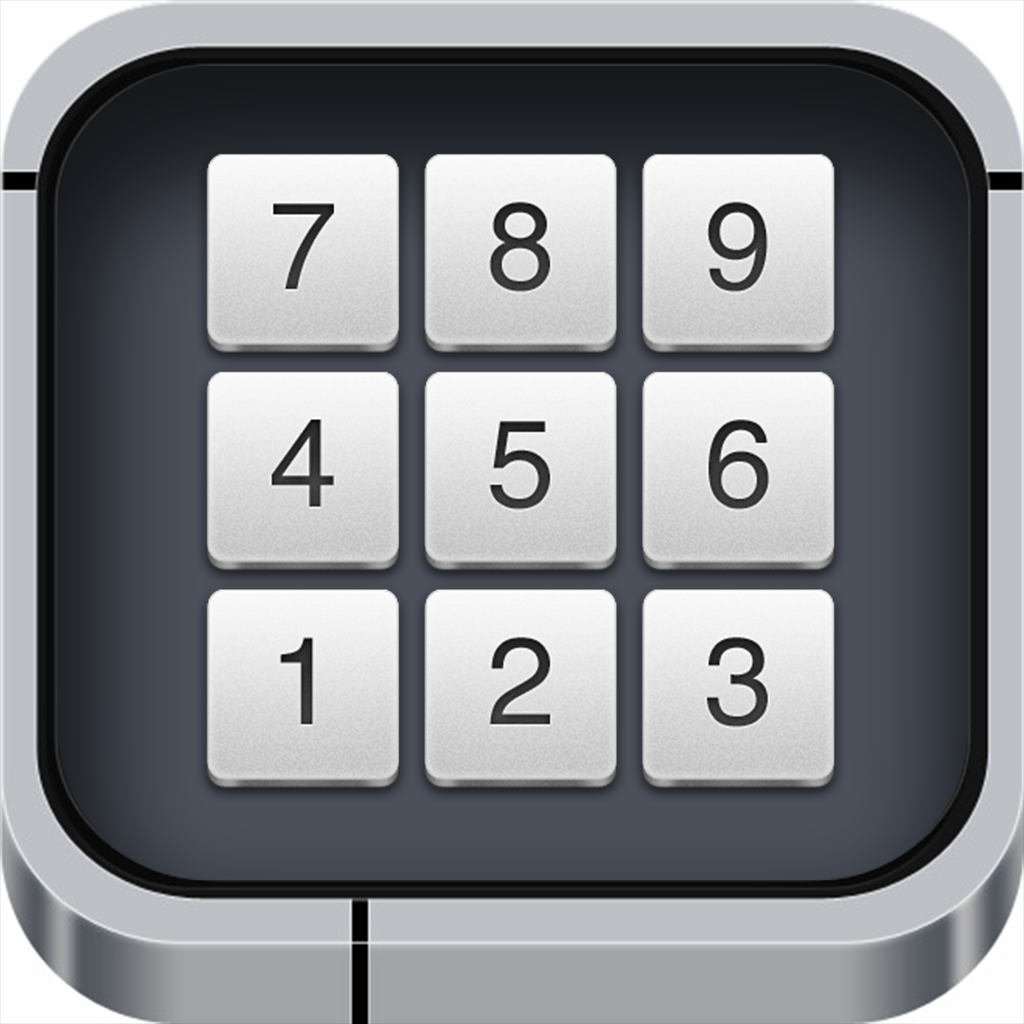
\includegraphics[width=4cm]{assets/1to9.png} \\
        % Change "assets/1to9.png" to "1to9.png" in polygon
    \end{center}


    You must choose a random message from box one which contains a string of some specific characters as the following:

    \begin{itemize}
        \item L: go to the left-side digit.
        \item R: go to the right-side digit.
        \item D: go to the down-side digit.
        \item U: go to the up-side digit.
    \end{itemize}

    And choose another random message from box two which has a number from $1$ to $9$ describe your start point.

\input

    You have two lines as the input.

    1st-line contains a string $s$ $(1 \le \vert s \vert \le 20000)$, message from box two $(1 \le n \le 9)$.

    2nd-line contains a message from box one (string $s$)

\output

    You need to print one single line containing the number of gifts you will take.

\note

    The numeric board is circular vertically and horizontally.